% Please do not change the document class
\documentclass{scrartcl}

% Please do not change these packages
\usepackage[hidelinks]{hyperref}
\usepackage[none]{hyphenat}
\usepackage{setspace}
\usepackage{graphicx}
\doublespace

% You may add additional packages here
\usepackage{amsmath}

% Please include a clear, concise, and descriptive title
\title{The Evaluation of Variation and Flexibility of Differing Procedural Content Generators for 2D Platform Games}

% Please do not change the subtitle
\subtitle{COMP110 - Computer Architecture Essay}

% Please put your student number in the author field
\author{1503048}

\begin{document}

\maketitle

\abstract{In this paper, three methods of procedural content generation shall be examined, in terms of the variation and flexibility of input provided. The overarching theme of recommendation is influenced by the application of each method with respect to the genre of 2D platform games. The intended recommendation is for an indie game development studio.}

\section{Introduction}

Procedural content generation (PCG) for games is a method of creating in-game objects and components. In terms of a 2D platformer, this can include components such as: enemies, gaps for the player to jump and platforms to land on. \\ \\
There are a number of issues to consider when using PCG, such as the cost effectiveness in comparison to a designer manually creating a level. However, in the scope of intended replayability, it is suitable for PCG use, due to its requirement of varied content generation.

Another issue with PCG is the playability of levels. While impressive in their generation, some levels are not functional due to improper placement of objects, i.e. the exit is placed out of reach of the player. \\ \\
The three main methods examined are: Smith et al's grammar-based approach using Launchpad \cite{Smith2011} ; Jennings-Teat’s et al's Polymorph using Dynamic Difficulty Adjustment (DDA) \cite{Jennings2010:Model} ; and Dahlskog et al's Multi-level Level Generator based on design patterns \cite{Dahlskog2014}.\\ \\
The metric used is the variation of generation and flexibility of input that each method provides. Furthermore, the conclusion should draw the paper towards a clear recommendation for implementation in a 2D platform game to be produced by an indie company.

\section{Methods}

\subsection{Introduction}

Launchpad is Smith et al's \cite{Smith2011} method for procedural content generation, for a 2D platformer level design. This design consists of a two-tiered, grammar-based approach. Their objective is for creating an autonomous, designer-guided level generator. It is a rhythm based level generator, where the term rhythm is explained through player pacing, movements and actions. For example, a player aims to match a series of actions with a rhythm of hitting the controller buttons in a speedrun behaviour \cite{Smith2011}.

Kremers theory of level design supports this necessity of maintaining pacing of a game, as it is described to be crucial to continual player engagement \cite[pp. 246]{Kremers2009}. \\ \\
Jennings-Teats et al \cite{Jennings2010:Model} discuss the use of Polymorph's dynamic level generation. This method is produced using Dynamic Difficulty Adjustment (DDA) which changes gameplay on-the-fly. This program aims to produce "continually-appropriate challenge" for its players \cite{Jennings2010:DDA}.

Similarly, it has been supported by Hunicke \cite{Hunicke2005}, that the appropriate level of difficulty for individual players is essential for enjoyment. \\ \\
Dahlskog et al's \cite{Dahlskog2014} approach uses a search-based, bottom-up approach. This method of builds on analysis of Super Mario Bros \cite{Dahlskog2012} levels into three levels of abstraction; using micro-, meso-, macro-patterns. These micro-patterns are used as the building blocks for the game producing vertical slices of the level which are then built into meso-patterns.

\subsection{Flexibility}

Launchpad allows the designer to manipulate a variety of parameters in order to give guidance and provide a rule set for the generator.

The parameter of rhythm can be manipulated through fields such as: evenly spaced beats, short followed by long beats or randomly spaced beats; these variables are also known as "regular", "swing" or "random" respectively \cite[pp. 7]{Smith2011}. 

\begin{figure}[h]
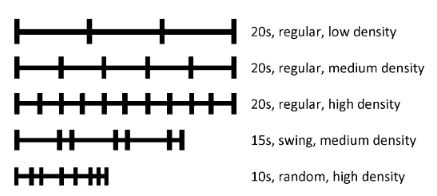
\includegraphics[width=11cm, height=5cm]{Smith_Fig1}
\centering
\caption{Examples of rhythm modification using type, density and length \cite{Smith2011}.}
\end{figure}
Fig. 1 shows examples of how the designer could modify the rhythm groups based on length, type and density. These rhythm groups are then translated into platforms and other geometry components within the game. \\  \\
The parameter input for Polymorph is based on player interaction. This not only allows for dynamic generation of adjacent components, but also the individual flexibility for personalised generation. Therefore, this method of DDA allows the designer to present the user with segments that are then assigned to levels by difficulty. \\ \\
Dahlskog et al's method of using a Multi-level Level Generator allows developers to create and analysis the difficulty of combined component groups present in these patterns. For example, creating groups such as: groups of enemies, gaps for the player to jump or valleys of varying levels \cite{Dahlskog2014}. 

Due to the bottom-up approach of this method, there is not much designer input, beyond the initial extracted sequence. The fitness function used measures the presence and order of existing patterns.

\subsection{Variation}

Launchpad's use of geometric interpretation of rhythm should be reflective of the designer input. This should then provide the player with varied geometric displays of rhythm. It also claims to uphold the integrity of the intended rhythm while still generating an "impressive variety of levels" \cite{Smith2011}. \\
\begin{figure}[h]
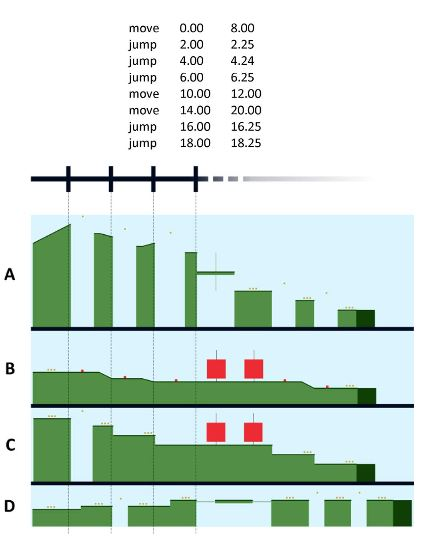
\includegraphics[width=7cm, height=9cm]{Smith_Fig2}
\centering
\caption{Four variations of geometric interpretation based on the same rhythm parameter set \cite{Smith2011}.}
\end{figure}

In Fig. 2, four levels are generated and directly comparable to the base rhythm set provided by the designer. The green platforms can be seen to fall or rise in line with the rhythm pace, as shown by the dotted lines. The large red squares in level B and C represent a stomper or a wait component. This has been interpreted in other variations, such as A and D, as a moving platform. It is debatable as to whether the intended rhythm is maintained. There is significant difference in player movement required at the beginning of segment B in comparison to segment A. \\ \\
Polymorph works by evaluating player behaviour through use of its learned model trained from its collected data. An applied Multilayer Perceptron algorithm is used to rank difficulty of generated level segments. In combination with the data collected from player's current performance, the next segment of the level is generated based on the player's behaviour.

\begin{figure}[h]
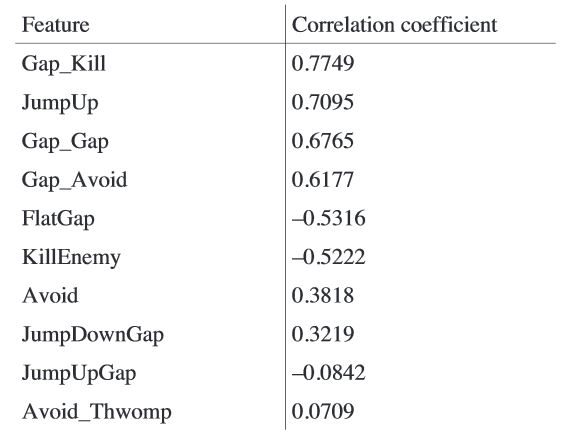
\includegraphics[width=11cm, height=9cm]{Jen_Fig2}
\centering
\caption{Correlation between level of difficulty rating and game component \cite{Jennings2010:Model}.}
\end{figure}

The data collected from gameplay, as shown in Fig. 3, has allowed the Polymorph model to assess the grouped and single components of a game based on difficulty. These results are then fed back into the next segment of the level to be generated and provide the player with appropriate difficulty. \\ \\
\begin{figure}[h]
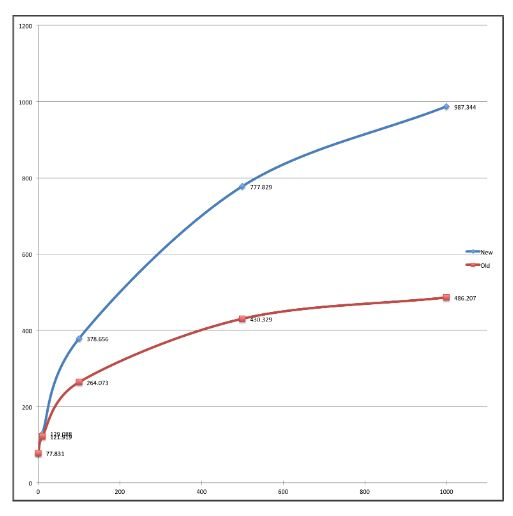
\includegraphics[width=11cm, height=9cm]{Dah_Fig1}
\centering
\caption{A comparison between the effects of mutation-operators between single (red) and five (blue) slice exchange \cite[pp. 4]{Dahlskog2014}.}
\end{figure}
The Multi-level Level Generator's uses a fitness function that allows "single-point mutation and one-point crossover" \cite[pp. 4]{Dahlskog2014}. This means that in 200 members, the 100 member of lowest fitness levels are discarded including those with unplayable content. The mutation basis for generated variation, operates through exchange of a set of five vertical slices "at a random starting position with a new random set of five slices" \cite[pp. 4]{Dahlskog2014}. This allows for greater variation between levels as larger segmented patterns are altered. This is shown in the steeper blue curve of Fig. 4 in comparison to the red line.

\section{Recommendation}

Launchpad provides a flexible generator, which allows the designer to clearly manipulate the pacing of the game level as intended with some reliability. 

Polymorph has shown to be a very successful data collection generator, allowing the results to dynamically adjust and generate gameplay through player interaction. This on-the-fly difficulty adjustments means a reduction in player frustration. 

Multi-level Level Generation has shown extensive experience with pattern deconstruction and combination. The mutation-operators have also shown effective in generator new content based on pattern replication and exchange. 

Overall, Polymorph's DDA approach provides a level balance of designer input and personalised level difficulty, with variation to generation. For an indie company, this reduces work load while still providing an enjoyable experience for players.


\bibliographystyle{ieeetr}
\bibliography{PCG_export}

\end{document}